% --------------------------------------------------------------
% This is all preamble stuff that you don't have to worry about.
% Head down to where it says "Start here"
% --------------------------------------------------------------
 
\documentclass[12pt]{article}
 
\usepackage[margin=1in]{geometry} 
\usepackage{amsmath,amsthm,amssymb,scrextend}
\usepackage{fancyhdr}
\usepackage{enumitem}
\usepackage{amsmath}
\usepackage{amssymb}
\usepackage{textcomp}
\usepackage{fancybox}
\usepackage{tikz}
\usepackage{tasks}
\pagestyle{fancy}
\usepackage[makeroom]{cancel}
\usepackage{graphicx}
\usepackage{caption}
\usepackage{mwe}


\usepackage{tikz}
\usetikzlibrary{positioning}

\newenvironment{rcases}
  {\left.\begin{aligned}}
{\end{aligned}\right\rbrace}

\newcommand{\N}{\mathbb{N}}
\newcommand{\Z}{\mathbb{Z}}
\newcommand{\I}{\mathbb{I}}
\newcommand{\R}{\mathbb{R}}
\newcommand{\Q}{\mathbb{Q}}
\renewcommand{\qed}{\hfill$\blacksquare$}
\let\newproof\proof
\renewenvironment{proof}{\begin{addmargin}[1em]{0em}\begin{newproof}}{\end{newproof}\end{addmargin}\qed}
% \newcommand{\expl}[1]{\text{\hfill[#1]}$}
 
\newenvironment{theorem}[2][Theorem]{\begin{trivlist}
\item[\hskip \labelsep {\bfseries #1}\hskip \labelsep {\bfseries #2.}]}{\end{trivlist}}
\newenvironment{lemma}[2][Lemma]{\begin{trivlist}
\item[\hskip \labelsep {\bfseries #1}\hskip \labelsep {\bfseries #2.}]}{\end{trivlist}}
\newenvironment{problem}[2][Problem]{\begin{trivlist}
\item[\hskip \labelsep {\bfseries #1}\hskip \labelsep {\bfseries #2.}]}{\end{trivlist}}
\newenvironment{exercise}[2][Exercise]{\begin{trivlist}
\item[\hskip \labelsep {\bfseries #1}\hskip \labelsep {\bfseries #2.}]}{\end{trivlist}}
\newenvironment{reflection}[2][Reflection]{\begin{trivlist}
\item[\hskip \labelsep {\bfseries #1}\hskip \labelsep {\bfseries #2.}]}{\end{trivlist}}
\newenvironment{proposition}[2][Proposition]{\begin{trivlist}
\item[\hskip \labelsep {\bfseries #1}\hskip \labelsep {\bfseries #2.}]}{\end{trivlist}}
\newenvironment{corollary}[2][Corollary]{\begin{trivlist}
\item[\hskip \labelsep {\bfseries #1}\hskip \labelsep {\bfseries #2.}]}{\end{trivlist}}




\setlength{\parindent}{0pt}
\begin{document}
\setcounter{section}{5}

 \settasks{
	counter-format=(tsk[r]),
	label-width=4ex
}
% --------------------------------------------------------------
%                         Start here
% --------------------------------------------------------------

\lhead{Math 475}
\chead{}
\rhead{Chapter 6}

\section{Inclusion - Exlusion}
\subsection{The Inclusion-Exclusion Principle}
{\sl Example}: Howmany integers from 1 through 600 are {\sl not} divisible by 6?\\ 
There are $\lfloor\frac{600}{6}\rfloor$ = 100 integers from 1 to 600 divisible by 6. By subtraction principle, there are 600-100 =500 {\sl not} divisible by 6.\\


\begin{center}
    


\tikzset{every picture/.style={line width=0.75pt}} %set default line width to 0.75pt        

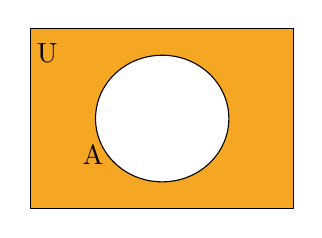
\begin{tikzpicture}[x=0.75pt,y=0.75pt,yscale=-1,xscale=1]
%uncomment if require: \path (0,541.6666564941406); %set diagram left start at 0, and has height of 541.6666564941406

%Shape: Rectangle [id:dp05587912413464302] 
\draw  [fill={rgb, 255:red, 245; green, 166; blue, 35 }  ,fill opacity=1 ] (265,367) -- (391.72,367) -- (391.72,454.02) -- (265,454.02) -- cycle ;
%Shape: Ellipse [id:dp12351413525185895] 
\draw  [fill={rgb, 255:red, 255; green, 255; blue, 255 }  ,fill opacity=1 ] (296.25,410.51) .. controls (296.25,393.67) and (310.63,380.01) .. (328.36,380.01) .. controls (346.1,380.01) and (360.48,393.67) .. (360.48,410.51) .. controls (360.48,427.36) and (346.1,441.01) .. (328.36,441.01) .. controls (310.63,441.01) and (296.25,427.36) .. (296.25,410.51) -- cycle ;

% Text Node
\draw (273,379) node  [align=left] {U};
% Text Node
\draw (295,428) node  [align=left] {A};


\end{tikzpicture}
\end{center}
\begin{itemize}
    \item[] $U = \{1,2,...,600\}$
    \item[] $A=\{x\in  U\;|\;6\;divides\;x\;evenly\}$
\end{itemize}

\vspace{1.5\baselineskip}
Given overlapping sets A and B (both subsets of A set $U$)
\begin{center}
\tikzset{every picture/.style={line width=0.75pt}} %set default line width to 0.75pt        

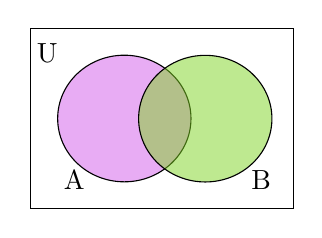
\begin{tikzpicture}[x=0.75pt,y=0.75pt,yscale=-1,xscale=1]
%uncomment if require: \path (0,541.6666564941406); %set diagram left start at 0, and has height of 541.6666564941406

%Shape: Rectangle [id:dp7039806797123567] 
\draw   (480,30) -- (606.72,30) -- (606.72,117.02) -- (480,117.02) -- cycle ;
%Shape: Ellipse [id:dp005629183715786912] 
\draw  [fill={rgb, 255:red, 189; green, 16; blue, 224 }  ,fill opacity=0.35 ] (493,73.5) .. controls (493,56.66) and (507.38,43) .. (525.12,43) .. controls (542.85,43) and (557.23,56.66) .. (557.23,73.5) .. controls (557.23,90.35) and (542.85,104) .. (525.12,104) .. controls (507.38,104) and (493,90.35) .. (493,73.5) -- cycle ;
%Shape: Ellipse [id:dp709858940130146] 
\draw  [fill={rgb, 255:red, 126; green, 211; blue, 33 }  ,fill opacity=0.5 ] (532,73.57) .. controls (532,56.72) and (546.38,43.06) .. (564.12,43.06) .. controls (581.85,43.06) and (596.23,56.72) .. (596.23,73.57) .. controls (596.23,90.41) and (581.85,104.07) .. (564.12,104.07) .. controls (546.38,104.07) and (532,90.41) .. (532,73.57) -- cycle ;

% Text Node
\draw (488,42) node  [align=left] {U};
% Text Node
\draw (501,103) node  [align=left] {A};
% Text Node
\draw (591,103) node  [align=left] {B};


\end{tikzpicture}
\end{center}
\begin{itemize}
    \item[] $|A\cup B| = |A|+|B|-|A\cap B|$
    \item[] $|\overline{A\cup B}| = |U|-|A|-|B|+|A\cap B|$
\end{itemize}

\vspace{1.5\baselineskip}
\begin{center}
\tikzset{every picture/.style={line width=0.75pt}} %set default line width to 0.75pt        

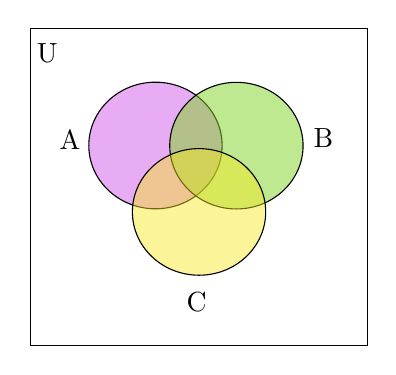
\begin{tikzpicture}[x=0.75pt,y=0.75pt,yscale=-1,xscale=1]
%uncomment if require: \path (0,541.6666564941406); %set diagram left start at 0, and has height of 541.6666564941406

%Shape: Rectangle [id:dp19955462080031805] 
\draw   (476,140) -- (638.23,140) -- (638.23,293.07) -- (476,293.07) -- cycle ;
%Shape: Ellipse [id:dp03567076164118688] 
\draw  [fill={rgb, 255:red, 189; green, 16; blue, 224 }  ,fill opacity=0.35 ] (504,196.5) .. controls (504,179.66) and (518.38,166) .. (536.12,166) .. controls (553.85,166) and (568.23,179.66) .. (568.23,196.5) .. controls (568.23,213.35) and (553.85,227) .. (536.12,227) .. controls (518.38,227) and (504,213.35) .. (504,196.5) -- cycle ;
%Shape: Ellipse [id:dp17834962514454733] 
\draw  [fill={rgb, 255:red, 126; green, 211; blue, 33 }  ,fill opacity=0.5 ] (543,196.57) .. controls (543,179.72) and (557.38,166.06) .. (575.12,166.06) .. controls (592.85,166.06) and (607.23,179.72) .. (607.23,196.57) .. controls (607.23,213.41) and (592.85,227.07) .. (575.12,227.07) .. controls (557.38,227.07) and (543,213.41) .. (543,196.57) -- cycle ;
%Shape: Ellipse [id:dp7300939460760469] 
\draw  [fill={rgb, 255:red, 248; green, 231; blue, 28 }  ,fill opacity=0.45 ] (525,228.5) .. controls (525,211.66) and (539.38,198) .. (557.12,198) .. controls (574.85,198) and (589.23,211.66) .. (589.23,228.5) .. controls (589.23,245.35) and (574.85,259) .. (557.12,259) .. controls (539.38,259) and (525,245.35) .. (525,228.5) -- cycle ;

% Text Node
\draw (484,152) node  [align=left] {U};
% Text Node
\draw (495,194) node  [align=left] {A};
% Text Node
\draw (617,193) node  [align=left] {B};
% Text Node
\draw (556,272) node  [align=left] {C};
\end{tikzpicture}
\end{center}
\begin{align*}
    |A\cup B\cup C| &= |A|+|B|+|C|-|A\cap B|-|A\cap C|-|B\cap C| +|A\cap B\cap C|\\
    |\overline{A\cup B\cup C}| &= |U| - |A|-|B|-|C|+|A\cap B|+|A\cap C|+|B\cap C| - |A\cap B\cap C|
\end{align*}

{\sl Example}: Find the number of integers from 1 to 1000 inclusive that are not divisible by 5,6, or 8. (i.e. not divisible by any of 5,6, and 8)


\begin{align*}
    \text{Let } &\text{$U$ = set of integers from 1 through 1000}\\
    &\text{$A_1$ = Set of integers in $U$ divisible by 5}\\
    &\text{$A_2$ = Set of integers in $U$ divisible by 6}\\
    &\text{$A_3$ = Set of integers in $U$ divisible by 8}
\end{align*}

We want to find $|\overline{A_1\cup A_2\cup A_3}| = |\overline{A}_1\cap\overline{A}_2\cap \overline{A}_3|$ (De Morgan's Law)\\

\begin{itemize}
    \item $U$ = 1000
    \item $|A_1|=\lfloor \frac{1000}{5}\rfloor =200$
    \item $|A_2| = \lfloor \frac{1000}{6}\rfloor = 166$
    \item $|A_3|=\lfloor \frac{1000}{8}\rfloor = 125$
    \item $|A_1\cap A_2| = \lfloor\frac{1000}{30}\rfloor = 33$
    \item $|A_1\cap A_3| = \lfloor\frac{1000}{40}\rfloor = 25$
    \item $|A_2\cap A_3| = \lfloor\frac{1000}{24} = 41$
    \item $|A_1\cap A_2 \cap A_3| = \lfloor \frac{1000}{120}\rfloor = 8$
    \item $|\overline{A_1 \cup A_2\cup A_3}| =$ 1000-200-166-125+33+25+41-8=600
\end{itemize}
\end{document}
